\newpage

%-------------------------------------------------%
%------------------------Α------------------------%
%-------------------------------------------------%

\begin{justify}
    {\bf Α.} Σε αυτήν την άσκηση, θα προσομοιώσουμε το τηλεπικοινωνιακό
    σύστημα του Σχήματος, υποθέτοντας ότι χρησιμοποιείται
    διαμόρφωση \textlatin{16-QAM}, και θα μελετήσουμε την
    απόδοσή του.
\end{justify}


%------------------------Α.1----------------------%
\begin{justify}
    {\bf 1.} Για δεδομένα Ν (ενδεικτικά Ν=200), να
    δημιουργήσετε δυαδική ακολουθία με στοιχεία
    4Ν ισοπίθανα \textlatin{bits}.
\end{justify}

\begin{justify}
    {\bf Λύση:}\\
    Ακολοθεί ο κώδικας \textlatin{MatLab}:
\end{justify}

\vspace{-1cm}

%---------------------MATLAB code-----------------%
\textlatin{
    \lstinputlisting[language=Matlab,]{ALPHA/Matlab/a1.m}
} 

%-------------------------------------------------%

%------------------------Α.2----------------------%
\begin{justify}
    {\bf 2.} (15) Να συντάξετε συνάρτηση
    \[
      X=bits\_to\_4PAM(bit\_seq,A)  
    \]
    η οποία, χρησιμοποιώντας κωδικοποίηση \textlatin{Gray},
    απεικονίζει την δυαδική ακολουθία σε εισόδου \textlatin{bit\_seq}
    σε ακολουθία \textlatin{4-PAM} συμβόλων.
\end{justify}

\begin{justify}
    {\bf Λύση:}\\
    Ακολοθεί ο κώδικας \textlatin{MatLab}:
\end{justify}

\vspace{-1cm}

%---------------------MATLAB code-----------------%
\textlatin{
    \lstinputlisting[language=Matlab,]{ALPHA/Matlab/a2.m}
} 

%-------------------------------------------------%

%------------------------Α.3----------------------%

\begin{justify}
    {\bf 3.} Να απεικονίσετε τα πρώτα 2Ν \textlatin{bits}
    της ακολουθίας του βήματος 1 στα \textlatin{4-PAM} 
    σύμβολα $X\textsubscript{1,\textlatin{n},}$ για 
    $n=1,...,N$. και τα επόμενα 2Ν \textlatin{bits}
    στα \textlatin{4-PAM} σύμβολα $X\textsubscript{\textlatin{Q},\textlatin{n},}$ για
    $n=1,...,N$.
\end{justify}

\begin{justify}
    {\bf Λύση:}\\
    Ακολοθεί ο κώδικας \textlatin{MatLab}:
\end{justify}

\vspace{-1cm}

%---------------------MATLAB code-----------------%
\textlatin{
    \lstinputlisting[language=Matlab,]{ALPHA/Matlab/a3.m}
} 

%-------------------------------------------------%

\newpage

%------------------------Α.4----------------------%
\begin{justify}
    {\bf 4.} (5) Να περάσετε τις ακολυθίες  $X\textsubscript{1,\textlatin{n},}$
    και $X\textsubscript{\textlatin{Q},\textlatin{n},}$ από τα
    \textlatin{SRRC} φίλτρα μορφοποίησης και υποθέτοντας περίοδο
    συμβόλου $T=0.01sec$, $over=10$, $T_s=\frac{T}{over}$, να σχιματίσετε
    και να σχεδιάσετε τις κυματομορφές εξόδου $\textlatin{X}_1 (t)$
    και $\textlatin{X}_\textlatin{Q} (t)$ και τα περιοδογράμματά τους.
\end{justify}

\begin{justify}
    {\bf Λύση:}\\
    Παρακάτω φαίνονται οι κυματομορφές:
\end{justify}

%-----------------------PLOT-a.4.1----------------%

\begin{center}
    \centering
    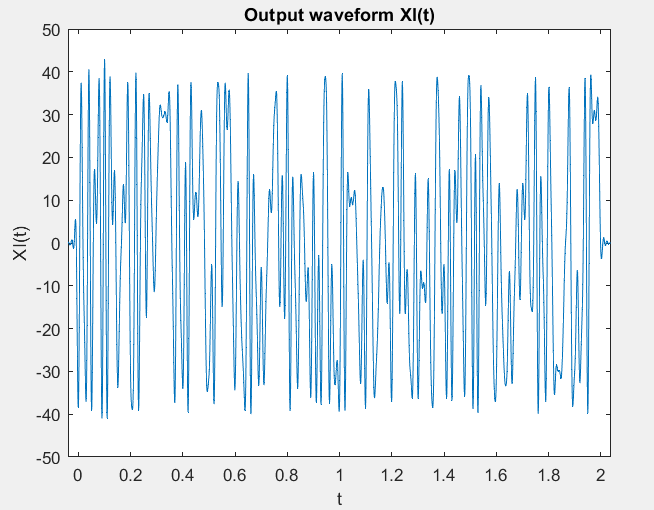
\includegraphics[width=0.8\textwidth]{ALPHA/IMAGES/a4.1.png} % Adjust width as neededfilename of your images
\end{center}

%-----------------------PLOT-a.4.2----------------%

\begin{center}
    \centering
    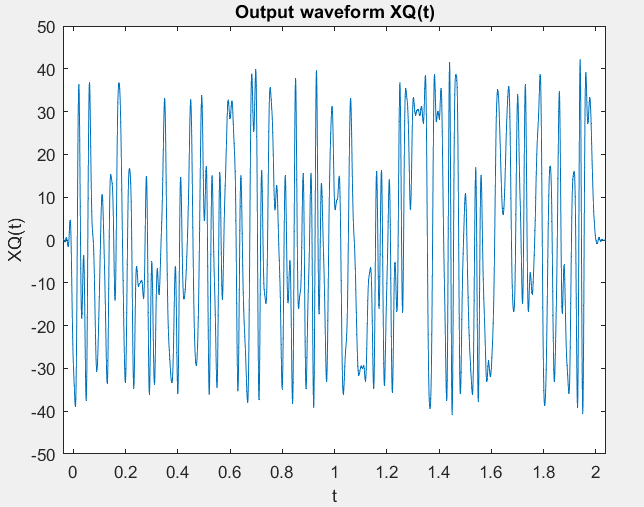
\includegraphics[width=0.8\textwidth]{ALPHA/IMAGES/a4.2.png} % Adjust width as neededfilename of your images
\end{center}

%-----------------------PLOT-a.4.3----------------%

\begin{center}
    \centering
    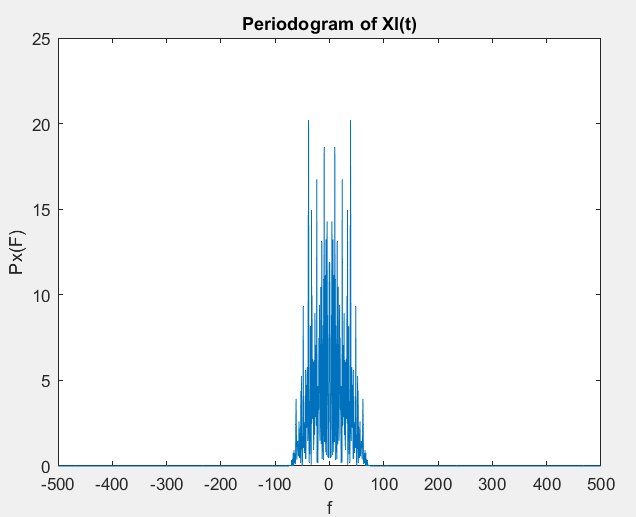
\includegraphics[width=0.8\textwidth]{ALPHA/IMAGES/a4.3.png} % Adjust width as neededfilename of your images
\end{center}


%-----------------------PLOT-a.4.4----------------%

\begin{center}
    \centering
    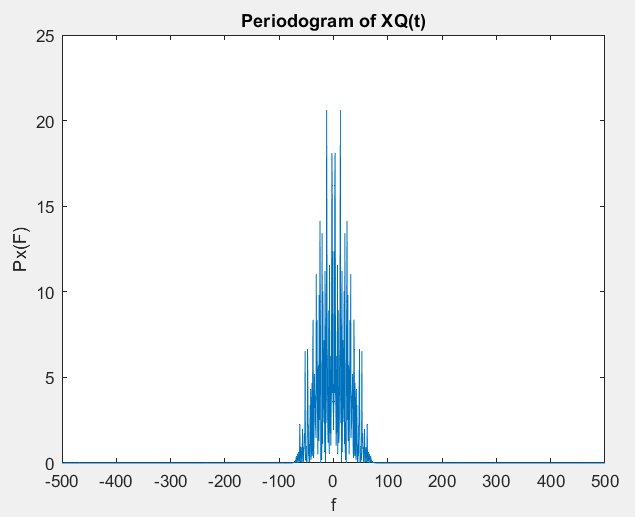
\includegraphics[width=0.8\textwidth]{ALPHA/IMAGES/a4.4.png} % Adjust width as neededfilename of your images
\end{center}



\begin{justify}
    Και ο κώδικας \textlatin{MatLab}:
\end{justify}

\vspace{-1cm}

%---------------------MATLAB code-----------------%
\textlatin{
    \lstinputlisting[language=Matlab,]{ALPHA/Matlab/a4.m}
} 

%-------------------------------------------------%

\newpage



%------------------------Α.5----------------------%

\begin{justify}
    {\bf 5.} (5) Να πολαπλασιάσετε τις κυματομορφές $\textlatin{X}_1 (t)$
    και $\textlatin{X}_\textlatin{Q} (t)$ με τους αντίστοιχους φορείς
    (ενδεικτικά $F_0=200 Hz$) και να δημιουργήσετε τις 
    κυματομορφές:
    \[
        \textlatin{X}_1\textsuperscript{\textlatin{mod}} (t)
        =2X_1(t)\cos(2\pi F_0 t), 
         \textlatin{X}_\textlatin{Q}\textsuperscript{\textlatin{mod}} (t)
        =-2X_\textlatin{Q}(t)\sin(2\pi F_0 t)
    \]
    Να σχεδιάσετε τις κυματομορφές που προκύπτουν καθώς και 
    τα αντίστοιχα περιοδογράμματα της. Τι παρατηρείτε\textlatin{;}

\end{justify}
\begin{justify}
    {\bf Λύση:}\\
    Κάνοντας τις κατάλληλες ενέργειες προκύπτουν οι κυματομορφές:
\end{justify}

%-----------------------PLOT-a.5.1----------------%

\begin{center}
    \centering
    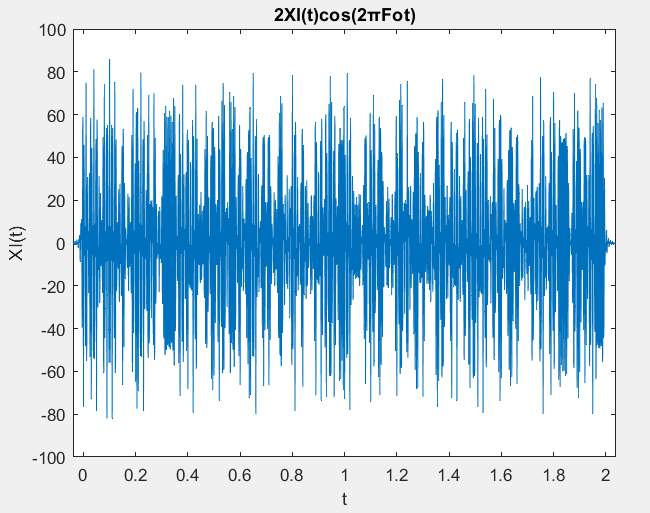
\includegraphics[width=0.8\textwidth]{ALPHA/IMAGES/a5.1.png} % Adjust width as neededfilename of your images
\end{center}

%-----------------------PLOT-a.5.2----------------%

\begin{center}
    \centering
    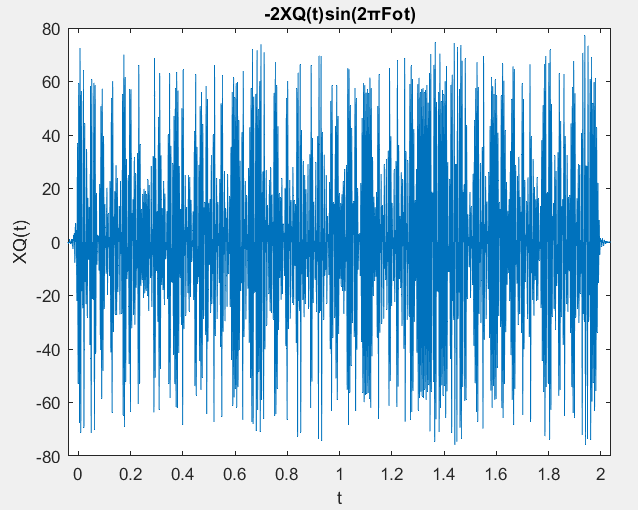
\includegraphics[width=0.8\textwidth]{ALPHA/IMAGES/a5.2.png} % Adjust width as neededfilename of your images
\end{center}

%-----------------------PLOT-a.5.3----------------%

\begin{center}
    \centering
    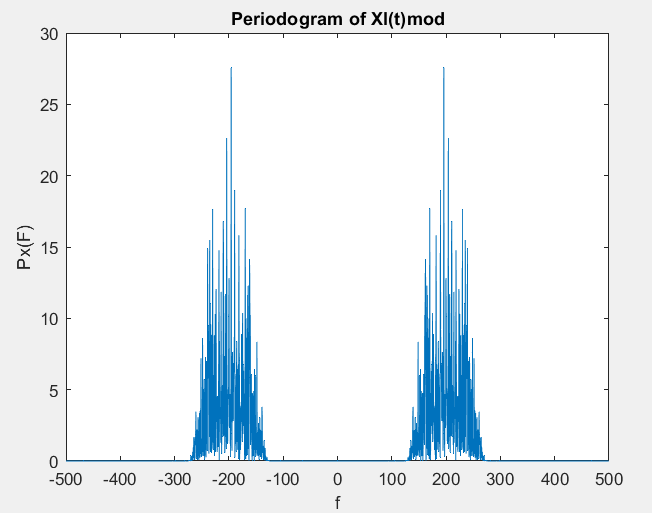
\includegraphics[width=0.8\textwidth]{ALPHA/IMAGES/a5.3.png} % Adjust width as neededfilename of your images
\end{center}


%-----------------------PLOT-a.5.4----------------%

\begin{center}
    \centering
    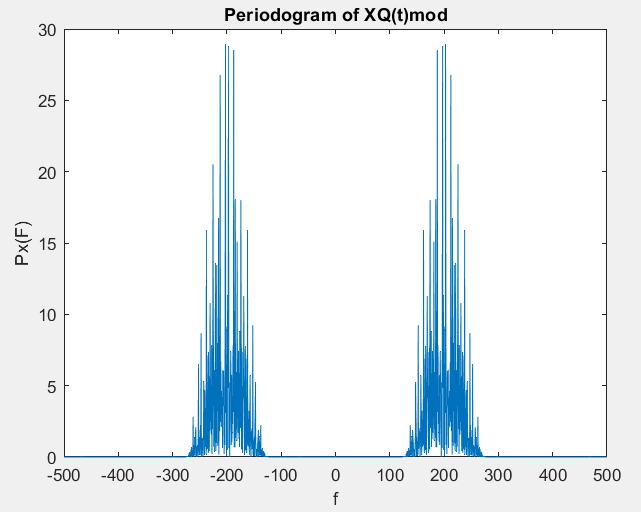
\includegraphics[width=0.8\textwidth]{ALPHA/IMAGES/a5.4.png} % Adjust width as neededfilename of your images
\end{center}


\begin{justify}
    Και ο κώδικας \textlatin{MatLab}:
\end{justify}

\vspace{-1cm}

%---------------------MATLAB code-----------------%
\textlatin{
    \lstinputlisting[language=Matlab,]{ALPHA/Matlab/a5.m}
} 

\begin{justify}
    Όπως παρατηρούμε από τα περιοδογράμματα, η διαμόρφωση
    έχει γίνει γύρο από την συχνότητα $\pm$ {\bf\textlatin{200Hz}}. 
\end{justify}

%-------------------------------------------------%

\newpage

%------------------------Α.6----------------------%


\begin{justify}
    {\bf 6.} (5) Να σχηματίσετε και να σχεδιάσετε
    την είσοδο του καναλιού,
    \[
        \textlatin{X}\textsuperscript{\textlatin{mod}} (t)
        =\textlatin{X}_1\textsuperscript{\textlatin{mod}} (t)
        +  \textlatin{X}_\textlatin{Q}\textsuperscript{\textlatin{mod}} (t) 
    \]
    και το περιοδογράμματά της. Τι παρατηρείτε\textlatin{;}
\end{justify}

\begin{justify}
    {\bf Λύση:}\\
   Προκύπτουν οι κυματομορφές:
\end{justify}
%-----------------------PLOT-a.6.1----------------%

\begin{center}
    \centering
    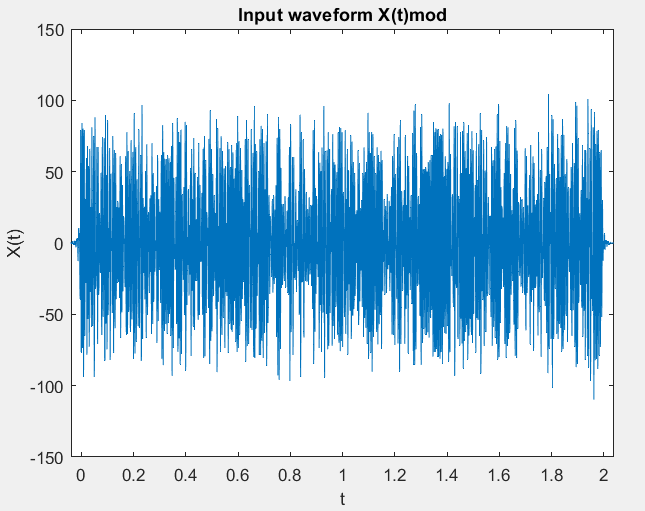
\includegraphics[width=0.8\textwidth]{ALPHA/IMAGES/a6.1.png} % Adjust width as neededfilename of your images
\end{center}

%-----------------------PLOT-a.6.2----------------%

\begin{center}
    \centering
    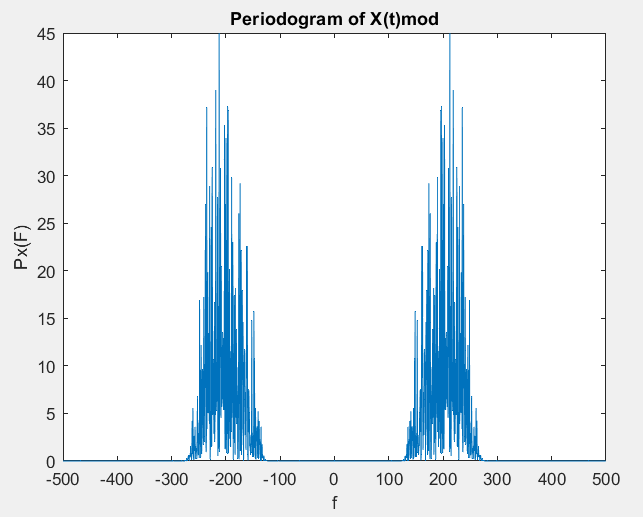
\includegraphics[width=0.8\textwidth]{ALPHA/IMAGES/a6.2.png} % Adjust width as neededfilename of your images
\end{center}


\begin{justify}
    Και ο κώδικας \textlatin{MatLab}:
\end{justify}

\vspace{-1cm}

%---------------------MATLAB code-----------------%
\textlatin{
    \lstinputlisting[language=Matlab,]{ALPHA/Matlab/a6.m}
} 

\begin{justify}
    Παρατηρώντας τα περιοδογράμματα, το πλάτος έχει αυξηθεί,
    πράγμα λογικό αφού πραγματοποιήσαμε πρόσθεση. Επιπλέον,
    όμοια με πριν η διαμόρφωση
    έχει γίνει γύρο από την συχνότητα $\pm$ {\bf\textlatin{200Hz}}.
\end{justify}

%-------------------------------------------------%

%------------------------Α.7----------------------%

\begin{justify}
    {\bf 7.} Να υποθέσετε ότι το κανάλι είναι
    ιδανικό.
\end{justify}

\begin{justify}
    {\bf Λύση:}\\
    Υποθέτουμε ότι το κανάλι είναι ιδανικό.
\end{justify}

%-------------------------------------------------%

%------------------------Α.8----------------------%

\begin{justify}
    {\bf 8.} (5) Στην έξοδο του καναλιού, να προσθέσετε λευκό \textlatin{Gaussian} θόρυβο 
    \( W(t) \) με διασπορά ίση με
    \[
     \sigma^2_W = \frac{10A^2}{T_s \cdot 10^{\frac{SNR_{dB}}{10}}}
    \]
\end{justify}

\begin{justify}
    {\bf Λύση:}\\
    Ακολοθεί ο κώδικας \textlatin{MatLab}:
\end{justify}

\vspace{-1cm}

%---------------------MATLAB code-----------------%
\textlatin{
    \lstinputlisting[language=Matlab,]{ALPHA/Matlab/a8.m}
} 

%-------------------------------------------------%

\newpage

%------------------------Α.9----------------------%

\begin{justify}
    {\bf 9.} (5) Στον δέκετη να διακλαδώσετε την ενθόρυβη
    κυματομορφή και να την πολαπλασιάσετε με φορείς
    $\cos(2\pi F_0 t)$ και $-\sin(2\pi F_0 t)$, αντίστοιχα.
    Να σχεδιάσετε τις κυματομορφές που προκύπτουν και τα 
    περιοδογράμματά τους. Τι παρατηρείτε\textlatin{;}
\end{justify}

\begin{justify}
    {\bf Λύση:}\\
    Προκύπτουν οι κυματομορφές:
\end{justify}

%-----------------------PLOT-a.9.1----------------%

\begin{center}
    \centering
    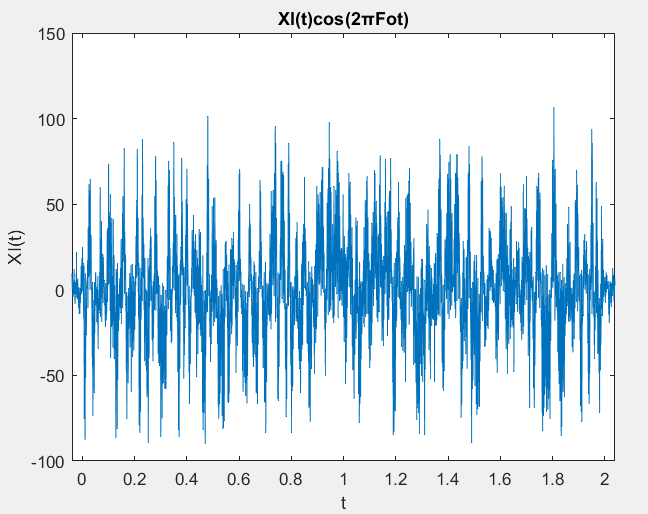
\includegraphics[width=0.8\textwidth]{ALPHA/IMAGES/a9.1.png} % Adjust width as neededfilename of your images
\end{center}

%-----------------------PLOT-a.9.2----------------%

\begin{center}
    \centering
    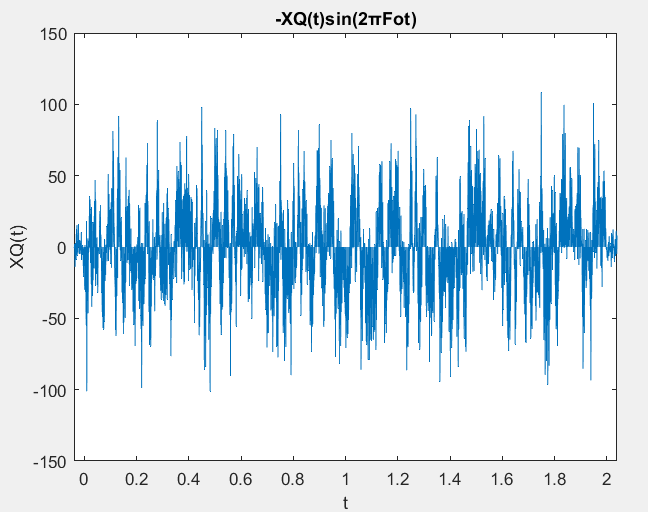
\includegraphics[width=0.8\textwidth]{ALPHA/IMAGES/a9.2.png} % Adjust width as neededfilename of your images
\end{center}

%-----------------------PLOT-a.9.2----------------%

\begin{center}
    \centering
    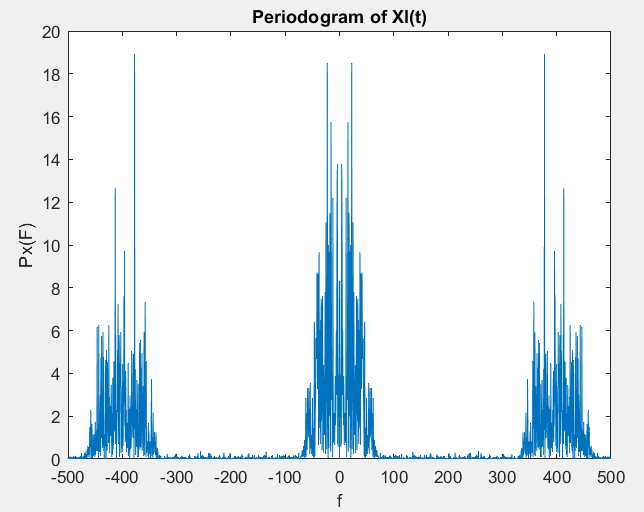
\includegraphics[width=0.8\textwidth]{ALPHA/IMAGES/a9.3.png} % Adjust width as neededfilename of your images
\end{center}

%-----------------------PLOT-a.9.4----------------%

\begin{center}
    \centering
    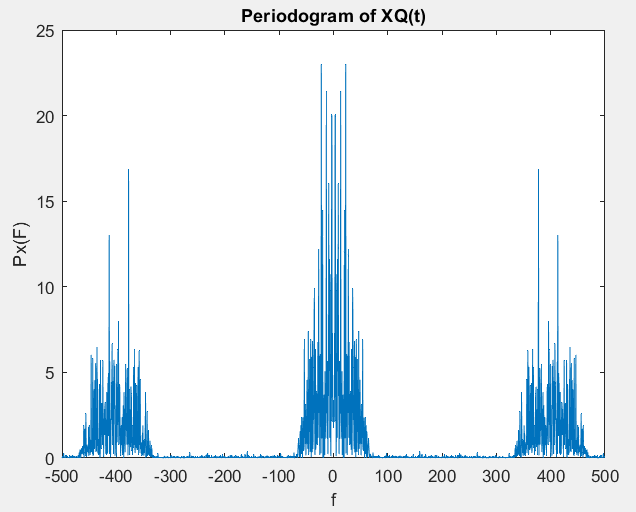
\includegraphics[width=0.8\textwidth]{ALPHA/IMAGES/a9.4.png} % Adjust width as neededfilename of your images
\end{center}

\begin{justify}
    Ακολοθεί ο κώδικας \textlatin{MatLab}:
\end{justify}

\vspace{-1cm}

%---------------------MATLAB code-----------------%
\textlatin{
    \lstinputlisting[language=Matlab,]{ALPHA/Matlab/a9.m}
} 

\begin{justify}
   Παρατηρούμε ότι τα περιοδογράμματα έχουν κέντρο
   τις συχνότητες {\bf $-F_0, 0, F_0$}.
\end{justify}

%-------------------------------------------------%

\newpage

%------------------------Α.10----------------------%

\begin{justify}
    {\bf 10.} (5) Να περάσετε τις κυματομορφές που
    υπολογίσατε στο προηγούμενο βήμα από τα προσαρμοσμένα
    φίλτρα. Να σχεδιάσετε τις κυματομορφές που προκύπτουν
    και τα περιοδογράμματά τους. Τι παρατηρείτε\textlatin{;}
\end{justify}

\begin{justify}
    {\bf Λύση:}\\
    Περνάμε τις κυματομορφές από φίλτρα και προκύπτουν:
\end{justify}

%-----------------------PLOT-a.10.1----------------%

\begin{center}
    \centering
    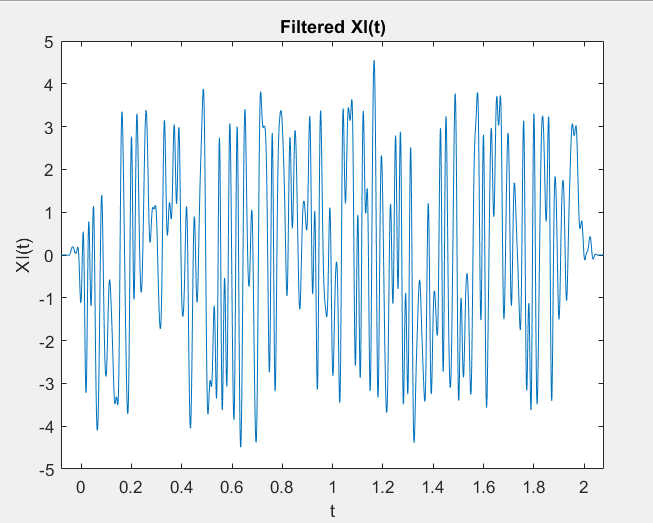
\includegraphics[width=0.8\textwidth]{ALPHA/IMAGES/a10.1.png} % Adjust width as neededfilename of your images
\end{center}

%-----------------------PLOT-a.10.2----------------%

\begin{center}
    \centering
    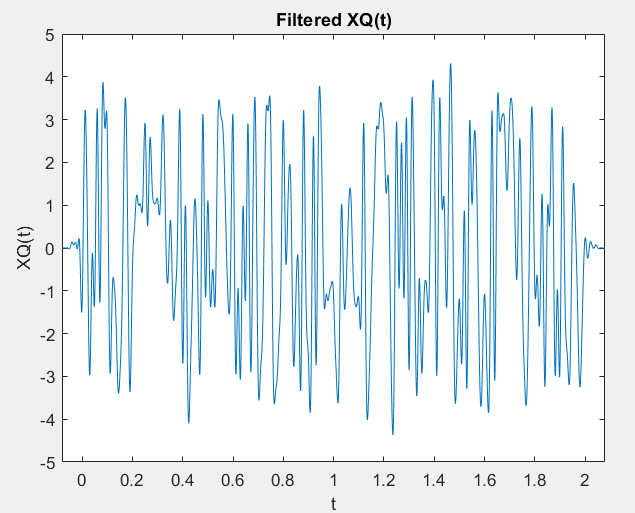
\includegraphics[width=0.8\textwidth]{ALPHA/IMAGES/a10.2.png} % Adjust width as neededfilename of your images
\end{center}

%-----------------------PLOT-a.10.3----------------%

\begin{center}
    \centering
    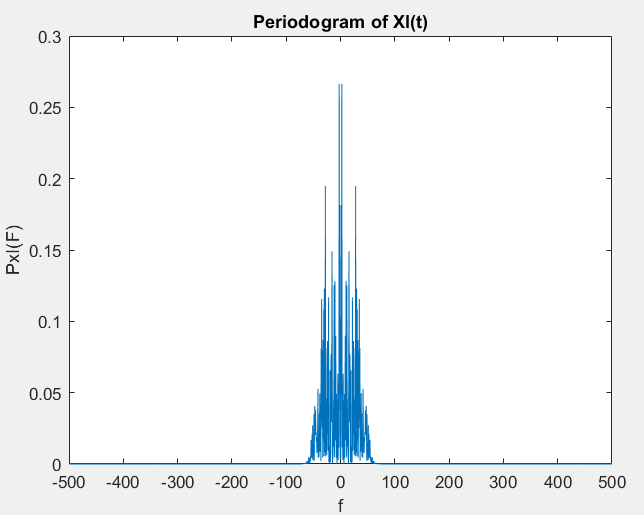
\includegraphics[width=0.8\textwidth]{ALPHA/IMAGES/a10.3.png} % Adjust width as neededfilename of your images
\end{center}

%-----------------------PLOT-a.10.4----------------%

\begin{center}
    \centering
    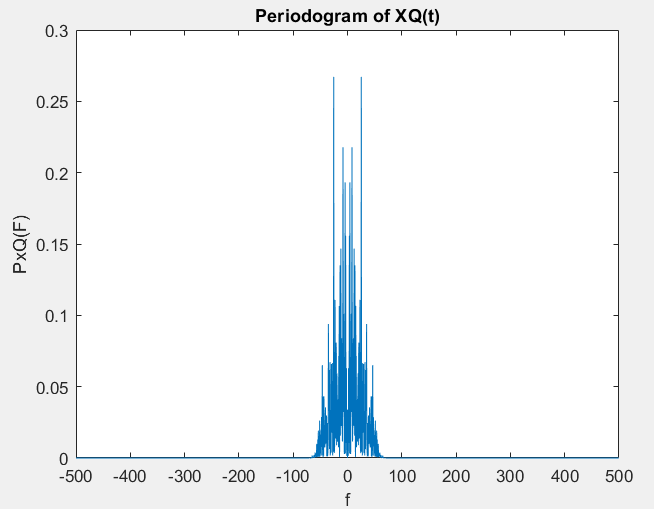
\includegraphics[width=0.8\textwidth]{ALPHA/IMAGES/a10.4.png} % Adjust width as neededfilename of your images
\end{center}

\begin{justify}
    Και ο κώδικας \textlatin{MatLab}:
\end{justify}

\vspace{-1cm}

%---------------------MATLAB code-----------------%

\textlatin{
    \lstinputlisting[language=Matlab,]{ALPHA/Matlab/a10.m}
}

\begin{justify}
    Όπως παρατηρούμε, μετά το φιλτράρισμα,έχουν αποκοπεί οι όροι στις μεγάλες
    συχνότητες.
\end{justify}

%-------------------------------------------------%

\newpage

%------------------------Α.11----------------------%

\begin{justify}
    {\bf 11.} (5) Να δειγματοληπτήσετε την έξοδο των προσαρμοσμένων
    φίλτρων τις κατάλληλες χρονικές στιγμές και να σχεδιάσετε
    την ακολουθία εξόδου χρησιμοποιώντας την εντολή
    \textlatin{scatterplot}.
\end{justify}

\begin{justify}
    {\bf Λύση:}\\\\
    Για \textlatin{SNR=10:}
\end{justify}

%-----------------------PLOT-a.11.1----------------%

\begin{center}
    \centering
    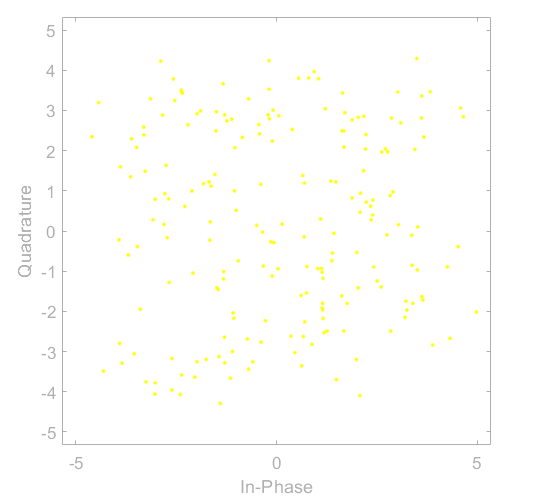
\includegraphics[width=0.8\textwidth]{ALPHA/IMAGES/a11.1.png} % Adjust width as neededfilename of your images
\end{center}

\newpage

\begin{justify}
    Και για \textlatin{SNR=20:}
\end{justify}

%-----------------------PLOT-a.11.2----------------%

\begin{center}
    \centering
    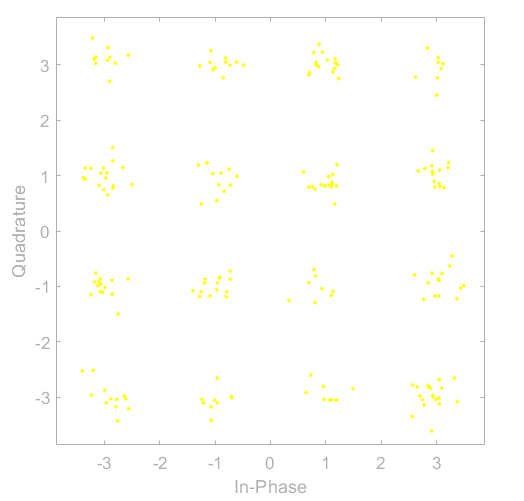
\includegraphics[width=0.8\textwidth]{ALPHA/IMAGES/a11.2.png} % Adjust width as neededfilename of your images
\end{center}

\begin{justify}
    Και ο κώδικας \textlatin{MatLab}:
\end{justify}

\vspace{-1cm}

%---------------------MATLAB code-----------------%

\textlatin{
    \lstinputlisting[language=Matlab,]{ALPHA/Matlab/a11.m}
}

%-------------------------------------------------%

\newpage

%------------------------Α.12----------------------%

\begin{justify}
    {\bf12.} (10) Να γράψετε την συνάρτηση:
    \[
      est\_X =  detect\_4\_PAM(Y,A)  
    \]
    η οποία χρησιμοποιεί τον κανόνα τον κανόνα εγγύτερου
    γείτονα και αποφασίζει για την ακολουθία εισόδου
    \textlatin{4-PAM} σύμβολο προς σύμβολο. Να εφαρμόσετε
    τη συνάρτηση ξεχωριστά στα δείγματα που λάβατε στην 
    \textlatin{inphase} έξοδο και στην \textlatin{quadtrature} έξοδο
    και να λάβετε αποφάσεις για τις αντίστοιχες ακολουθίες
    εισόδου.
\end{justify}

\begin{justify}
    {\bf Λύση:}\\
    Ο κώδικας \textlatin{MatLab} για την συνάρτηση
    \textlatin{detect\_4\_PAM}:
\end{justify}

\vspace{-1cm}

%---------------------MATLAB code-----------------%

\textlatin{
    \lstinputlisting[language=Matlab,]{ALPHA/Matlab/detect_4_PAM.m}
}

\begin{justify}
    Και έπειτα την εφαρμόζουμε στις δειγματοληπτημένες
    εξόδους του προηγούμενου ερωτήματος:
\end{justify}

\vspace{-1cm}

%---------------------MATLAB code-----------------%

\textlatin{
    \lstinputlisting[language=Matlab,]{ALPHA/Matlab/a12.m}
}

%-------------------------------------------------%

\newpage

%------------------------Α.13----------------------%

\begin{justify}
    {\bf 13.} (10) Χρησιμοποιώντας τις ακολουθίες εισόδου
    και τις αποφάσεις, να υπολογίσετε τον αριθμό σφαλμάτων
    απόφασης συμβόλου για τον αστερισμό \textlatin{16-QAM}. 
\end{justify}

\begin{justify}
    {\bf Λύση:}\\
    Για να υπολογιστεί ο αριθμός σφαλμάτων απόφασης συμβόλου,
    τοποθετήθακαν σε πίνακες οι αρχικές ακολουθίες εισόδου
    και οι αποφάσεις. Τέλος συγκρίνεται η διαφορά τους και αν αυτή
    είναι διαφορετική του μηδενός, υπάρχει σφάλμα απόφασης.
    Για \textlatin{SNR=10} το σφάλμα είναι {\bf 50} ενώ για 
    \textlatin{SNR=20} το σφάλμα είναι {\bf 0}. Αυτό είναι λογικό
    αφού για μεγαλύτερο \textlatin{SNR} λαμβάνουμε περισσότερη
    πληροφορία.
\end{justify}

\begin{justify}
    Ο κώδικας \textlatin{MatLab} για τον υπολογισμό:
\end{justify}

\vspace{-1cm}

%---------------------MATLAB code-----------------%

\textlatin{
    \lstinputlisting[language=Matlab,]{ALPHA/Matlab/a13.m}
}
%-------------------------------------------------%


%------------------------Α.14----------------------%

\begin{justify}
    {\bf 14.} (10) Να γράψετε την συνάρτηση:
    \[
      est\_bit = PAM\_4\_to\_bits(X,A)  
    \]
    η οποία χρησιμοποιεί την αντίστροφη απεικόνιση
    \textlatin{Gray}, δηλαδή, από σύμβολα σε δυάδες
    \textlatin{bits}, και από τις αποφάσεις για τις ακολουθίες
    συμβόλων εισόδου υπολογίζει την εκτιμώμενη δυαδική ακολουθία
    εισόδου. 
\end{justify}

\begin{justify}
    {\bf Λύση:}\\
    Κατασκευάστηκε η συνάρτηση \textlatin{PAM\_4\_to\_bits}: 
\end{justify}

\vspace{-1cm}

%---------------------MATLAB code-----------------%

\textlatin{
    \lstinputlisting[language=Matlab,]{ALPHA/Matlab/PAM_4_to_bits.m}
}

%-------------------------------------------------%

%------------------------Α.15----------------------%

\begin{justify}
    {\bf 15.} (10) Να υπολογίσετε τον αριθμό σφμαλμάτων
    \textlatin{bit}.
\end{justify}

\begin{justify}
    {\bf Λύση:}\\
    Για να υπολογιστεί ο αριθμός σφαλμάτων \textlatin{bit},
    υπολογίστηκε η εκτιμώμενη ακολουθία εισόδου και συγκρίθηκε
    με την αρχική δυαδική ακολουθία. Για \textlatin{SNR=10}
    το σφάλμα είναι {\bf 394} ενώ για \textlatin{SNR=20} το σφάλμα
    είναι {\bf 386}.
\end{justify}

%---------------------MATLAB code-----------------%

\textlatin{
    \lstinputlisting[language=Matlab,]{ALPHA/Matlab/a15.m}
}


%-------------------------------------------------%
